\documentclass[a4paper]{article}

%% Language and font encodings
\usepackage{polski}
\usepackage[polish]{babel}
\usepackage[utf8x]{inputenc}
\usepackage[T1]{fontenc}
\usepackage{pdfpages}
\usepackage{indentfirst}
\usepackage{listings}

% Adjust penalties
\brokenpenalty=1000
\clubpenalty=1000
\widowpenalty=1000

%% Sets page size and margins
\usepackage[a4paper]{geometry}

%% Useful packages
\usepackage{amsmath}
\usepackage{graphicx}
\usepackage[colorlinks=true, allcolors=blue]{hyperref}
\usepackage{booktabs}
\usepackage{cancel}
\usepackage{tikz}

\usepackage{float}

\renewcommand\thesection{\arabic{section}.}
\renewcommand\thesubsection{\arabic{section}.\arabic{subsection}.}
\renewcommand\thesubsubsection{\arabic{section}.\arabic{subsection}.\arabic{subsubsection}.}

% The following commands are not supported in PSTricks at present
% We define them conditionally, so when they are implemented,
% this pgf file will use them.
\ifx\du\undefined
  \newlength{\du}
\fi
\setlength{\du}{15\unitlength}

\newcommand{\Vsp}[1]{\vtop to #1 {}}
\newcommand{\Hsp}[1]{\hbox to #1 {}}
\newcommand{\Small}{\scriptsize}

\title{Sprawozdanie nr 1}
\date{}


\begin{document}

\begin{center}
\begin{tabular}{|p{5.5cm}|l|l|c|}
    \hline
	% Row 1.1  
	    Wydział \Vsp{4mm} &
	    \multicolumn{1}{|l}{Dzień} &
	    poniedziałek $17^{15} - 19^{30}$ &
	    Nr zespołu \\
	% Row 1.2
	    \mbox{\small{Matematyki i Nauk Informatycznych}} &
	    \multicolumn{1}{|l}{Data}  &
	    &
	    \multicolumn{1}{c|}{\Large{18}} \\
    
    \hline
	% Row 2.1 
	    Nazwisko i Imię: &
	    \Small Ocena z przygotowania &
	    \Small Ocena ze sprawozdania &
	    \Small Ocena Końcowa \\
	% Rows 2.2-2.4
	    1. Jasiński Bartosz & & &\\
	    2. Sadłocha Adrian & & & \\
	    3. Wódkiewicz Andrzej & & & \\

    \hline
    % Row 3.1
	    \multicolumn{2}{|l|}{Prowadzący \Vsp{4mm}} &
	    \multicolumn{2}{|l|}{Podpis prowadzącego} \\  
    % Row 3.2
    	\multicolumn{2}{|l|}{dr hab. Katarzyna Grebieszkow} &
    	\multicolumn{2}{|l|}{} \\    	
    \hline
\end{tabular}
\label{pieczatka}
\end{center}

{\let\newpage\relax\maketitle}  % stolen from: https://tex.stackexchange.com/questions/86249/maketitle-text-before-title
\setcounter{secnumdepth}{2}


\section{Opis ćwiczenia}
Ćwiczenie złożone było z dwóch części:
\begin{enumerate}
	\item{Badanie anharmoniczności drgań wahadła matematycznego}
	\item{Wyznaczanie przyspieszenia ziemskiego za pomocą wahadła różnicowego}
\end{enumerate}


\subsection{Wstęp teoretyczny}

\textbf{Wahadłem matematycznym płaskim} nazywamy punkt materialny, poruszający się po
fragmęcie okregu w jednorodnym polu grawitacyjnym. Praktyczną realizacją tego pojęcia
jest obciążnik (najczęściej kulka) o małych rozmiarach, zamocowany na nierozciągliwej
nici o bardzo małej, pomijalnej masie (Rysunek \ref{wahadlo_matematyczne}).

%\begin{figure}[h!]
%\centering
%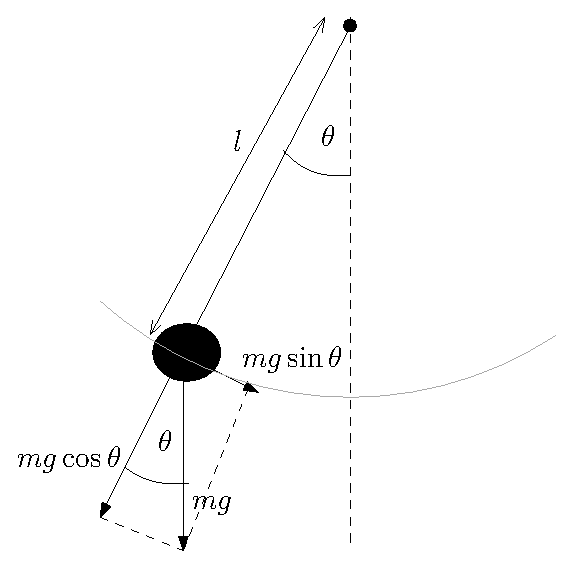
\includegraphics[scale=0.8]{wahadlo.eps}
%\caption{Wahadło matematyczne}
%\label{wahadlo_matematyczne}
%\end{figure}

Siłę ciężkości $\vec{F}_g = m\vec{g}$ działającą na ciężarek możemy rozłożyć na
składową radialną $F_g \cos \theta$ oraz styczną do toru ruchu wahadła $F_g \sin \theta$.
Składowa styczna wpływa na zmianę wektora prędkości ciężarka, gdyż działa ona
zawsze przeciwnie do jego wychylenia. Z drugiej zasady dynamiki Newtona mamy więc:

\begin{align*}
 ma &= -mg\sin\theta \\
 \frac{d^2S}{dt^2} &= -g\sin\theta
\end{align*}

Ponieważ $S = l \cdot \theta$:

\[ \frac{d^2\theta}{dt^2} = -\frac{g}{l}\sin\theta \]


Nie istnieje analityczne rozwiązanie tego równania różniczkowego. Dla małych kątów
można uprościć powyższy wzór, zakładając, że \, $\sin\theta \approx \theta$ \,
-- wtedy równanie różniczkowe daje się rozwiązać analitycznie. W rezultacie otrzymujemy,
że \textbf{dla wahadła matematycznego poruszającego się w zakresie małych kątów}
(przy założeniu $\theta(0) = \theta_{max}$):

\[ \theta(t) = \theta_{max}\cos\left(\sqrt{\frac{g}{l}}\,t\right), \]

czyli ruch \textbf{jest harmoniczny}, a okres tego ruchu wynosi

\[ T = 2\pi~\sqrt{\frac{l}{g}} \]


W ogólności (bez założenia małych wychyleń), korzystając z rozwinięcia funkcji $sin$
w szereg, możemy finalnie otrzymać zależność okresu drgań wahadła $T$ od kąta
maksymalnego wychylenia $\theta_{max}$:
\begin{equation} \label{eq:T}
T = 2\pi ~ \sqrt[]{\frac{l}{g}}~f(\theta_{max}) ,
\end{equation}
\begin{equation} \label{eq:f}
\text{gdzie} \enskip  \enskip f(\theta_{max}) = 
	\sum\limits_{n=0}^{\infty} 
		\left[ \frac{(2n)!}{(2^nn!)^2} \right]^2 
			\sin^{2n}\left(\frac{\theta_{max}}{2} \right)
\end{equation}


Ruch wahadła matematycznego jest więc w ogólności \textbf{anharmoniczny} -- okres
jest zależny od amplitudy.

\textbf{Wahadło różnicowe} to wahadło w którym mamy możliwość zmiany długości nici na której 
jest zawieszony ciężarek, pozwalające
mierzyć w precyzyjny sposób zmianę jej długości, nie znając długości bezwzględnej. Wykonując dwa pomiary $T_1, T_2$ dla różnych długości wahadła $l_1, l_2$ otrzymujemy:

\[ T^2_1 - T^2_2 = \frac{4\pi ^2}{g}\left(l_1-l_2\right) f(\theta_{max}) \]

\subsection{Układ pomiarowy}
Do przeprowadzenia obu części ćwiczenia posłużono się układem pomiarowym,
przedstawionym na rysunku \ref{uklad_pomiarowy}. Do ruchomego elementu 
połączonego z nieruchomym statywem przymocowana była długa, nierozciągliwa nitka, 
o znikomo małej masie, z zamocowanym na jej końcu metalowym obciążnikiem. 
Statyw pozwalał na modyfikowanie długość wahadła. Do statywu 
przytwierdzony był również kątomierz oraz linijka, służące do pomiaru kolejno:
kąta maksymalnego wychylenia wahadła oraz zmiany długości wahadła różnicowego.
Pod statywem znajdował się elektroniczny układ pomiarowy, złożony z fotokomórki
oraz modułu sterowania, za pomocą którego mierzony był okres wahadła.


%\begin{figure}[h]
%\centering
%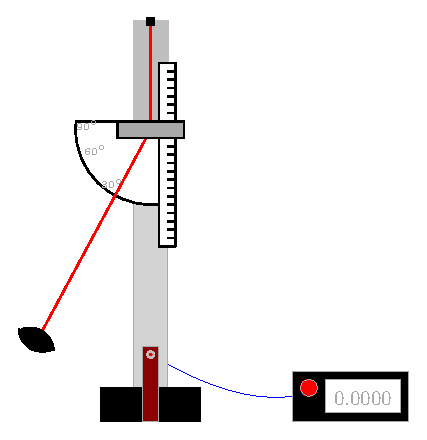
\includegraphics[scale=1]{uklad.eps}
%\caption{Schemat układu pomiarowego}
%\label{uklad_pomiarowy}
%\end{figure}


\section{Pomiary i obliczenia}
\subsection{Badanie zależności okresu drgań wahadła od kąta wychylenia}

Dokonano po 10 pomiarów dwóch okresów wahadła dla sześciu różnych kątów maksymalnego wychylenia wahadła. 
Wartości kątów wynosiły kolejno:
$5^\circ, 10^\circ, 15^\circ, 20^\circ, 25^\circ$ i $30^\circ$. 
Wyniki pomiarów znajdują się w tabeli \ref{pomiary_1}. Sporządzono również dwa wykresy: 
wartości średniej dwóch okresów wahadła względem kąta maksymalnego wychylenia oraz 
odchylenia standardowego pomiaru dla danego kąta (kolejno rysunki \ref{fig:mean}, \ref{fig:std}).

Długość wahadła nie była znana eksperymentatorom -- linijka używana w układzie pomiarowym
nie wskazywała bezwzględnej długości nici (służyła do odczytywania zmian długości nici wahadła różnicowego). 
Dlatego też w tym doświadczeniu nie można było wykorzystać zmierzonej wartości okresu
wahadła do wyliczenia przyspieszenia ziemskiego.

Z wykresu na rysunku \ref{fig:mean} można wywnioskować, że po pierwsze: \textbf{istnieje nie stała} funkcja długości okresu wahadła od kąta maksymalnego wychylenia (wartość średnia nie jest stała dla kolejnych kątów) oraz po drugie: funkcja ta jest \textbf{nieliniowa}. 
Uzyskane wyniki są zgodne z rozważaniami teoretycznymi (patrz wzór (\ref{eq:T})).


\begin{table}[h!]
\centering
	\begin{tabular}{rrrrrrr}
	\toprule
	{} &$2T(\alpha=5^\circ)$ &$2T(10^\circ)$ &$2T(15^\circ)$ &$2T(20^\circ)$ &$2T(25^\circ)$ &$2T(30^\circ)$ \\
	\midrule
	1 &  2.6285 &  2.6343 &  2.6368 &  2.6454 &  2.6585 &  2.6701 \\
	2 &  2.6295 &  2.6346 &  2.6359 &  2.6463 &  2.6589 &  2.6711 \\
	3 &  2.6295 &  2.6344 &  2.6402 &  2.6467 &  2.6582 &  2.6714 \\
	4 &  2.6307 &  2.6366 &  2.6394 &  2.6470 &  2.6590 &  2.6709 \\
	5 &  2.6296 &  2.6358 &  2.6408 &  2.6467 &  2.6578 &  2.6701 \\
	6 &  2.6286 &  2.6350 &  2.6404 &  2.6463 &  2.6593 &  2.6685 \\
	7 &  2.6285 &  2.6342 &  2.6396 &  2.6463 &  2.6574 &  2.6698 \\
	8 &  2.6303 &  2.6350 &  2.6401 &  2.6477 &  2.6588 &  2.6696 \\
	9 &  2.6287 &  2.6352 &  2.6395 &  2.6476 &  2.6583 &  2.6694 \\
	10 &  2.6298 &  2.6350 &  2.6396 &  2.6485 &  2.6584 &  2.6708 \\
	\midrule
	$2\overline{T}$& 2.62937 & 2.63501 & 2.63923 & 2.64685 & 2.64685 & 2.67017 \\ 
	$s(2T)$ & 0.00078 & 0.00074 & 0.00160 & 0.00089 & 0.00057 & 0.00089 \\
	\bottomrule
\end{tabular}
\caption{Seria pomiarów czasu trwania 2 okresów wahadła w zależności od kąta wychylenia}
\label{pomiary_1}
\end{table}

%\begin{figure}[h!]
%\centering
%	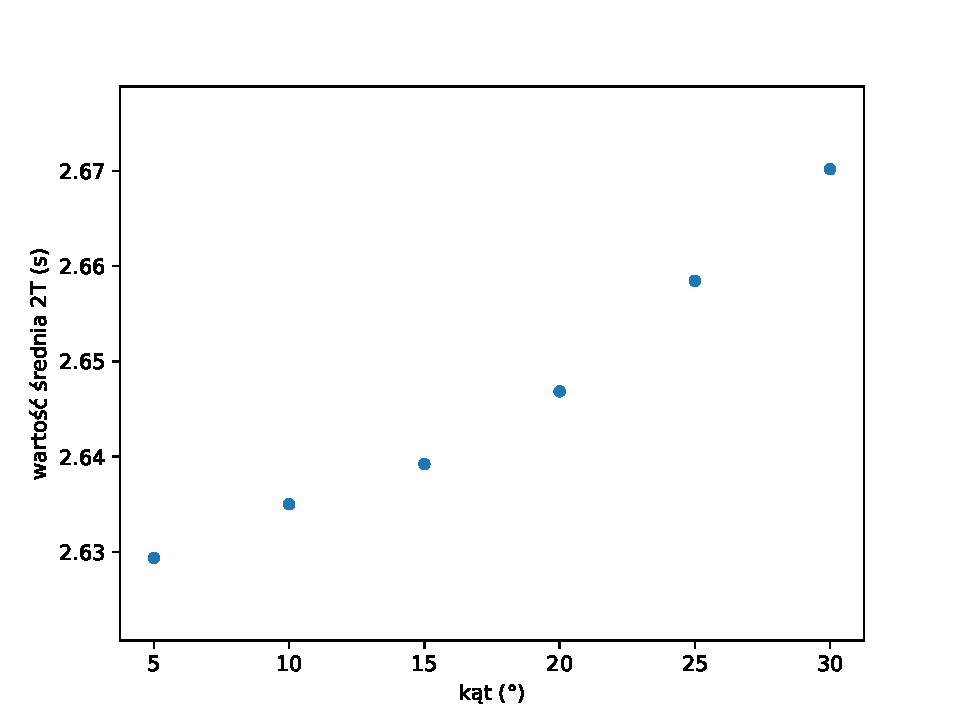
\includegraphics[scale=0.7]{wykres-1_0.pdf}
%\caption{Wartość średnia 2 okresów wahadła w zależności od maksymalnego kąta wychylenia}
%\label{fig:mean}
%\end{figure}

Nie zaobserwowano natomiast żadnej zależności między odchyleniem standardowym pomiarów 
a kątem maksymalnego wychylenia (rysunek \ref{fig:std}).


%\begin{figure}[h!]
%\centering
%	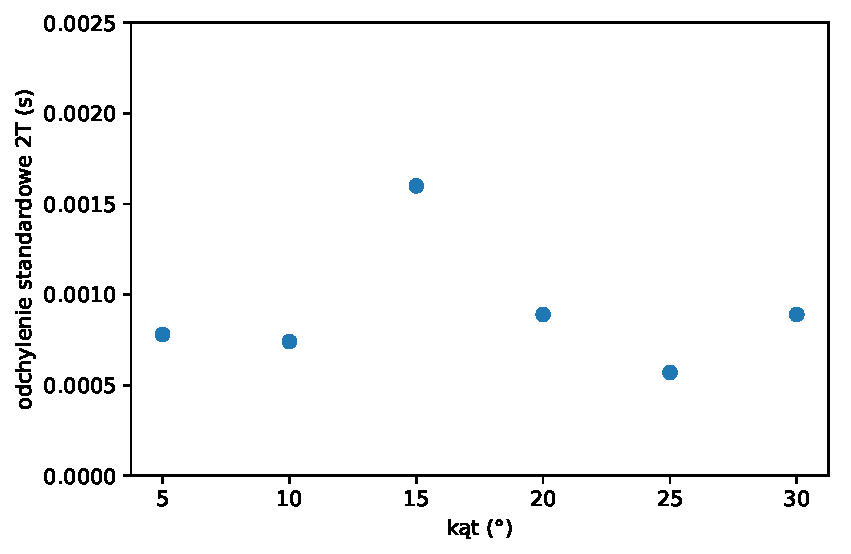
\includegraphics[scale=0.7]{wykres-2_1.pdf}
%\caption{Odchylenie standardowe 2 okresów wahadła w zależności od maksymalnego kąta wychylenia}
%\label{fig:std}
%\end{figure}


\subsection{Badanie zależności okresu drgań od zmian długości wahadła}

Przekształcając wzór (\ref{eq:T})  otrzymujemy zależność:
\[l = g\frac{T^2}{4\pi^2}\frac{1}{f^2(\theta_{max})} \]
Dalej, korzystając z podstawienia \[g' = \frac{g}{f^2(\theta_{max})} \]
oraz z faktu, że odczytywana z linijki długość wahadła nie jest jego rzeczywistą długością --
wartości na linijce zmieniają się \textbf{odwrotnie proporcjonalnie} do długości wahadła --
otrzymujemy finalnie:
\begin{equation} \label{eq:l_wzg}
 l_{odczyt} = -g'\frac{T^2}{4\pi^2}
\end{equation}

W ten sposób po dokonaniu pomiarów okresu przy zmiennej długości wahadła można skorzystać z regresji liniowej i wyznaczyć nachylenie prostej, a w rezultacie wartość $g$.

\subsubsection{Pomiary okresu dla małego kąta}

Po przeprowadzeniu pomiarów dla kąta $\theta_{max} = 10^\circ$ dokonano wyznaczenia 
przyspieszenia ziemskiego przy użyciu metody najmniejszych kwadratów. 
Wyniki pomiarów wraz z obliczeniami cząstkowymi oraz oznaczenia $X$, $Y$ znajdują się w tabeli \ref{pomiary_2}.
W celu wyznaczenia współczynników regresji liniowej, jak i ich niepewności pomiarowych skorzystano ze wzorów:
\begin{align*}
a &= \frac{n \Sigma X Y - \Sigma X \Sigma Y}{n \Sigma X^2 - \left(\Sigma X\right)^2} \\
b &= \frac{1}{n}\left(\Sigma Y - a \Sigma X\right) \\
u(a) &= \sqrt{\frac{n}{n-2} \frac{\Sigma Y^2 - a\Sigma XY - b\Sigma Y}{n\Sigma X^2-\left(\Sigma X \right)^2}} \\
u(b) &= u(a)\cdot \sqrt{\frac{\Sigma X^2}{n}}
\end{align*}

Uzyskane wartości wyniosły: $a = -9.789(31)$  , \ $b = 909.4(1.5)$,
zatem przekształcając $a$ zgodnie ze wzorem (\ref{eq:l_wzg}):  \[g' = 9.789(31)  \tfrac{m}{s^2}\]

Ponieważ kąt maksymalnego wychylenia jest dostatecznie mały oraz z powodów dydaktycznych ćwiczenia,
w tym kroku doświadczenia celowo pominięto korektę na anharmoniczność.

\begin{table}[h!]
\centering
	\begin{tabular}{lrrrrrr}
	\toprule
	{} & $l$ (mm) $=Y$ &  $2T$ (s) & \small$1000T^2/4\pi^2$\normalsize$=X (s^2)$ & $X^2$ & $Y^2$ & $XY$ \\
	\midrule
	1 &     480 &  2.6325 &  43.885094 &  1925.9015 &  230400 &  21064.845 \\
	2 &     460 &  2.6918 &  45.884484 &  2105.3859 &  211600 &  21106.863 \\
	3 &     440 &  2.7515 &  47.942349 &  2298.4688 &  193600 &  21094.634 \\
	4 &     420 &  2.8101 &  50.006196 &  2500.6196 &  176400 &  21002.602 \\
	5 &     400 &  2.8676 &  52.073578 &  2711.6575 &  160000 &  20829.431 \\
	6 &     380 &  2.9218 &  54.060647 &  2922.5536 &  144400 &  20543.046 \\
	\midrule
	$\Sigma$ & 2580 & 16.6753 & 293.852348 & 14464.5869 & 1116400 & 125641.421 \\
	\end{tabular}
\caption{Pomiary 2 okresów wahadła dla maksymalnego kąta wychylenia $\theta_{max} = 10^\circ$ w  zależności od $l$ wraz z obliczeniami do wyznaczenia regresji liniowej}
\label{pomiary_2}
\end{table}


%\begin{figure}[h!]
%\centering
%	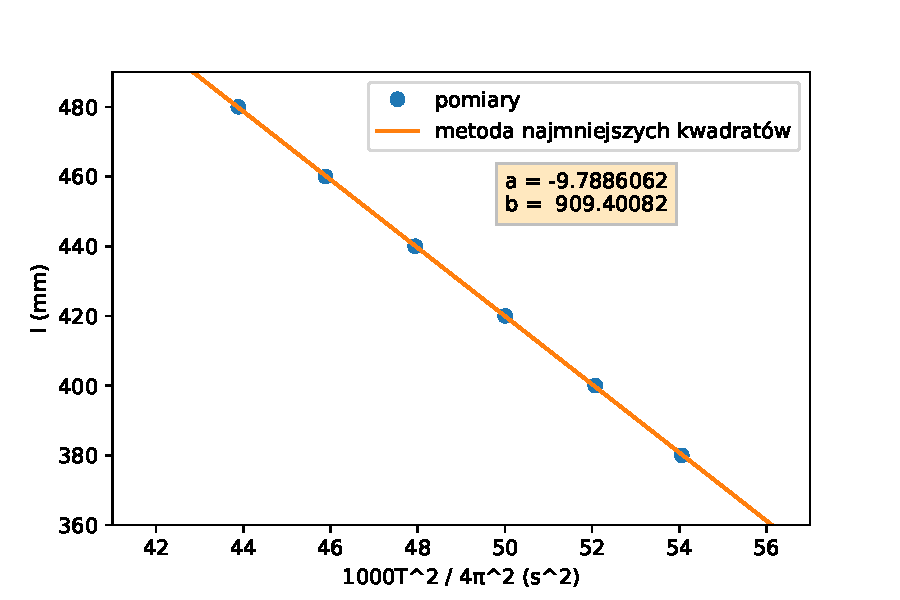
\includegraphics[scale=0.6]{wykres-3_0.pdf}
%\caption{Regresja liniowa metodą najmniejszych kwadratów dla $\theta_{max} = 10^\circ$}
%\label{regresja_10}
%\end{figure}


\subsubsection{Pomiary okresu dla dużego kąta}

Następnie dokonano pomiarów dla kąta $\theta_{max} = 25^\circ$. 
Dokonano analogicznych obliczeń (patrz Tabela \ref{pomiary_3}).
Uzyskane wartości parametrów prostej to: $a = -9.658(23)$, $b = 911.6(1.1)$,
zatem \[g' = 9.658(23)  \tfrac{m}{s^2}\]

Korzystając z korekty na anharmoniczność drgań dla pierwszych 3 wyrazów szeregu ze wzoru~(\ref{eq:f})
\[ K(\theta_{max}) = \left( 1 + \frac{1}{16}\theta^2_{max} + \frac{11}{3072}\theta^4_{max} + ... \right) \]
uzyskujemy: \[ g = g' \cdot 1.0120289 \approx 9.773(23) \tfrac{m}{s^2}\]



\begin{table}[h]
\centering

	\begin{tabular}{lrrrrrr}
	\toprule
		{} & $l$ (mm) $=Y$ &  $2T$ (s) & \small$1000T^2/4\pi^2$\normalsize$=X (s^2)$ & $X^2$ & $Y^2$ & $XY$ \\
	\midrule
	1 &     480 &  2.6582 &  44.74614 &  2002.2170 &  230400 &  21478.147 \\
	2 &     460 &  2.7160 &  46.71322 &  2182.1249 &  211600 &  21488.081 \\
	3 &     440 &  2.7764 &  48.81399 &  2382.8056 &  193600 &  21478.136 \\
	4 &     420 &  2.8339 &  50.85683 &  2586.4132 &  176400 &  21359.869 \\
	5 &     400 &  2.8918 &  52.95620 &  2804.3591 &  160000 &  21182.480 \\
	6 &     380 &  2.9494 &  55.08681 &  3034.5566 &  144400 &  20932.988 \\
	\midrule
	$\Sigma$ & 2580 & 16.8257 & 299.17319& 14992.4764 & 1116400 & 127919.701 \\
	\bottomrule
	\end{tabular}
	
\caption{Pomiary 2 okresów wahadła dla maksymalnego kąta wychylenia $\theta_{max} = 25^\circ$ w  zależności od $l$ wraz z obliczeniami do wyznaczenia regresji liniowej}
\label{pomiary_3}
\end{table}

%\begin{figure}[h]
%\centering
%	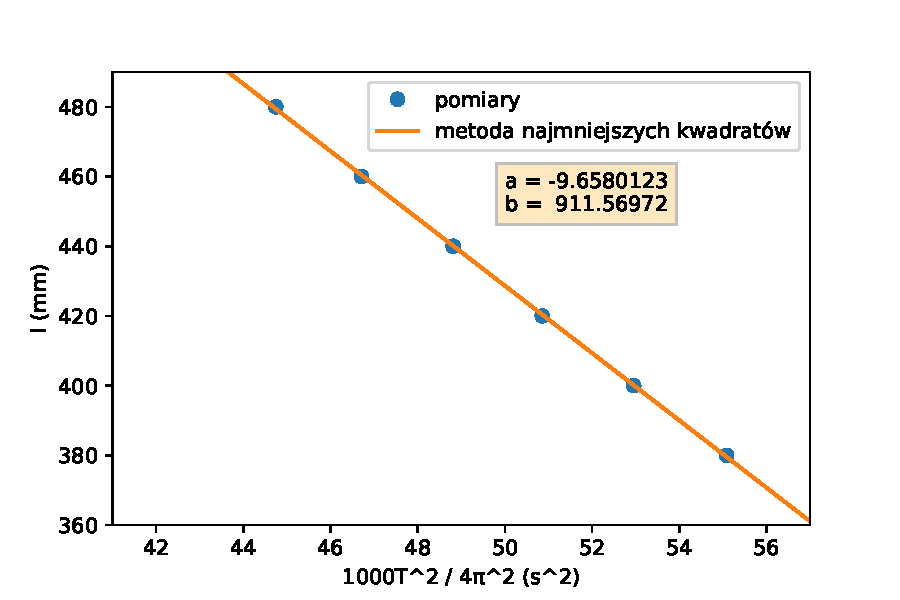
\includegraphics[scale=0.6]{wykres-4_0.pdf}
%\caption{Regresja liniowa metodą najmniejszych kwadratów dla $\theta_{max} = 25^\circ$}
%\label{regresja_25}
%\end{figure}


\subsection{Wnioski}
Po wykonaniu obu ćwiczeń potwierdzono anharmoniczność ruchu wahadła matematycznego oraz uzyskano
2 wartości przyspieszenia ziemskiego: $9.789(31) \tfrac{m}{s^2}$ oraz $9.773(23) \tfrac{m}{s^2}$.

Znając wartość przyspieszenia ziemskiego w Warszawie ($g\approx9,8123 \tfrac{m}{s^2}$)
można zauważyć, że w drugim ćwiczeniu pomimo zastosowania korekty na anharmoniczność drgań
przy serii pomiarów dla dużego kąta ($\theta_{max} = 25^\circ$), uzyskana wartość
przyspieszenia ziemskiego była mniej dokładna niż wartość uzyskana bez zastosowania
korekty przy serii pomiarów dla kąta mniejszego ($\theta_{max} = 10^\circ$).
Oznacza to, że niedoskonałości sprzętu pomiarowego i błędy eksperymentatorów znacznie
wpłynęły na wyniki pomiarów.
To przypuszczenie dodatkowo potwierdza kształt wykresu odchylenia standardowego
z pierwszego ćwiczenia (rysunek \ref{fig:std}).


Aby zmniejszyć niedoskonałości pomiarów należałoby zadbać o dokładniejszy sposób odczytu
kąta maksymalnego wychylenia wahadła (wyeliminować zjawisko paralaksy) oraz dodać do
układu pomiarowego możliwość mechanicznego zwalniania obciążnika wahadła, eliminując tym
samym przypadki zarówno wprawienia wahadła w ruch w 2 płaszczyznach 
jak i nadawania mu prędkości początkowej.


\end{document}
